\documentclass[a4paper,14pt, unknownkeysallowed]{extreport}

\usepackage{cmap} % Улучшенный поиск русских слов в полученном pdf-файле
\usepackage[T2A]{fontenc} % Поддержка русских букв
\usepackage[utf8]{inputenc} % Кодировка utf8
\usepackage[english,russian]{babel} % Языки: русский, английский
\usepackage{enumitem}


\usepackage{threeparttable}

\usepackage[14pt]{extsizes}

\usepackage{caption}
\captionsetup{labelsep=endash}
\captionsetup[figure]{name={Рисунок}}

% \usepackage{ctable}
% \captionsetup[table]{justification=raggedleft,singlelinecheck=off}

\usepackage{amsmath}

\usepackage{geometry}
\geometry{left=30mm}
\geometry{right=10mm}
\geometry{top=20mm}
\geometry{bottom=20mm}

\usepackage{titlesec}
\titleformat{\section}
	{\normalsize\bfseries}
	{\thesection}
	{1em}{}
\titlespacing*{\chapter}{0pt}{-30pt}{8pt}
\titlespacing*{\section}{\parindent}{*4}{*4}
\titlespacing*{\subsection}{\parindent}{*4}{*4}

\usepackage{setspace}
\onehalfspacing % Полуторный интервал

\frenchspacing
\usepackage{indentfirst} % Красная строка

\usepackage{titlesec}
\titleformat{\chapter}{\LARGE\bfseries}{\thechapter}{20pt}{\LARGE\bfseries}
\titleformat{\section}{\Large\bfseries}{\thesection}{20pt}{\Large\bfseries}

\usepackage{multirow}
\usepackage{listings}
\usepackage{xcolor}

% Для листинга кода:
\lstset{%
	language={c++},   					% выбор языка для подсветки	
	basicstyle=\small\sffamily,			% размер и начертание шрифта для подсветки кода
	numbers=left,						% где поставить нумерацию строк (слева\справа)
	numberstyle=\tiny,		   		% размер шрифта для номеров строк
	stepnumber=1,						% размер шага между двумя номерами строк
	numbersep=5pt,						% как далеко отстоят номера строк от подсвечиваемого кода
	frame=single,						% рисовать рамку вокруг кода
	tabsize=4,							% размер табуляции по умолчанию равен 4 пробелам
	captionpos=t,						% позиция заголовка вверху [t] или внизу [b]
	breaklines=true,					
	breakatwhitespace=true,				% переносить строки только если есть пробел
	backgroundcolor=\color{white},
	basicstyle=\footnotesize\ttfamily,
	keywordstyle=\color{blue},
	stringstyle=\color{red},
	commentstyle=\color{gray}
	showspaces=false,
    showstringspaces=false
}


\usepackage{pgfplots}
\usetikzlibrary{datavisualization}
\usetikzlibrary{datavisualization.formats.functions}


\lstset{
	literate=
	{а}{{\selectfont\char224}}1
	{б}{{\selectfont\char225}}1
	{в}{{\selectfont\char226}}1
	{г}{{\selectfont\char227}}1
	{д}{{\selectfont\char228}}1
	{е}{{\selectfont\char229}}1
	{ё}{{\"e}}1
	{ж}{{\selectfont\char230}}1
	{з}{{\selectfont\char231}}1
	{и}{{\selectfont\char232}}1
	{й}{{\selectfont\char233}}1
	{к}{{\selectfont\char234}}1
	{л}{{\selectfont\char235}}1
	{м}{{\selectfont\char236}}1
	{н}{{\selectfont\char237}}1
	{о}{{\selectfont\char238}}1
	{п}{{\selectfont\char239}}1
	{р}{{\selectfont\char240}}1
	{с}{{\selectfont\char241}}1
	{т}{{\selectfont\char242}}1
	{у}{{\selectfont\char243}}1
	{ф}{{\selectfont\char244}}1
	{х}{{\selectfont\char245}}1
	{ц}{{\selectfont\char246}}1
	{ч}{{\selectfont\char247}}1
	{ш}{{\selectfont\char248}}1
	{щ}{{\selectfont\char249}}1
	{ъ}{{\selectfont\char250}}1
	{ы}{{\selectfont\char251}}1
	{ь}{{\selectfont\char252}}1
	{э}{{\selectfont\char253}}1
	{ю}{{\selectfont\char254}}1
	{я}{{\selectfont\char255}}1
	{А}{{\selectfont\char192}}1
	{Б}{{\selectfont\char193}}1
	{В}{{\selectfont\char194}}1
	{Г}{{\selectfont\char195}}1
	{Д}{{\selectfont\char196}}1
	{Е}{{\selectfont\char197}}1
	{Ё}{{\"E}}1
	{Ж}{{\selectfont\char198}}1
	{З}{{\selectfont\char199}}1
	{И}{{\selectfont\char200}}1
	{Й}{{\selectfont\char201}}1
	{К}{{\selectfont\char202}}1
	{Л}{{\selectfont\char203}}1
	{М}{{\selectfont\char204}}1
	{Н}{{\selectfont\char205}}1
	{О}{{\selectfont\char206}}1
	{П}{{\selectfont\char207}}1
	{Р}{{\selectfont\char208}}1
	{С}{{\selectfont\char209}}1
	{Т}{{\selectfont\char210}}1
	{У}{{\selectfont\char211}}1
	{Ф}{{\selectfont\char212}}1
	{Х}{{\selectfont\char213}}1
	{Ц}{{\selectfont\char214}}1
	{Ч}{{\selectfont\char215}}1
	{Ш}{{\selectfont\char216}}1
	{Щ}{{\selectfont\char217}}1
	{Ъ}{{\selectfont\char218}}1
	{Ы}{{\selectfont\char219}}1
	{Ь}{{\selectfont\char220}}1
	{Э}{{\selectfont\char221}}1
	{Ю}{{\selectfont\char222}}1
	{Я}{{\selectfont\char223}}1
}

\usepackage{graphicx}
\newcommand{\img}[3] {
	\begin{figure}[h!]
		\center{\includegraphics[height=#1]{img/#2}}
		\caption{#3}
		\label{img:#2}
	\end{figure}
}


\usepackage[justification=centering]{caption} % Настройка подписей float объектов

\usepackage[unicode,pdftex]{hyperref} % Ссылки в pdf
\hypersetup{hidelinks}

\usepackage{csvsimple}

\newcommand{\code}[1]{\texttt{#1}}





\begin{document}


\begin{titlepage}
	\newgeometry{pdftex, left=2cm, right=2cm, top=2.5cm, bottom=2.5cm}
	\fontsize{12pt}{12pt}\selectfont
	\noindent \begin{minipage}{0.15\textwidth}
		
\includegraphics[width=\linewidth]{img/b_logo.jpg}
	\end{minipage}
	\noindent\begin{minipage}{0.9\textwidth}\centering
		\textbf{Министерство науки и высшего образования Российской Федерации}\\
		\textbf{Федеральное государственное бюджетное образовательное учреждение высшего образования}\\
		\textbf{«Московский государственный технический университет имени Н. Э.~Баумана}\\
		\textbf{(национальный исследовательский университет)»}\\
		\textbf{(МГТУ им. Н. Э.~Баумана)}
	\end{minipage}
	
	\noindent\rule{18cm}{3pt}
	\newline\newline
	\noindent ФАКУЛЬТЕТ $\underline{\text{«Информатика и системы управления»~~~~~~~~~~~~~~~~~~~~~~~~~~~~~~~~~~~~~~~~~~~~~~~~~~~~~~~}}$ \newline\newline
	\noindent КАФЕДРА $\underline{\text{«Программное обеспечение ЭВМ и информационные технологии»~~~~~~~~~~~~~~~~~~~~~~~}}$\newline\newline\newline\newline\newline\newline\newline
	
	
	\begin{center}
		\noindent\begin{minipage}{1.3\textwidth}\centering
		\Large\textbf{   ~~~ Лабораторная работа №5}\newline
		\textbf{по дисциплине "Анализ Алгоритмов"}\newline\newline\newline
		\end{minipage}
	\end{center}
	
	\noindent\textbf{Тема} 			$\underline{\text{Конвейерная обработка данных}}$\newline\newline
	\noindent\textbf{Студент} 		$\underline{\text{Ковалец К. Э.}}$\newline\newline
	\noindent\textbf{Группа} 		$\underline{\text{ИУ7-53Б}}$\newline\newline
	\noindent\textbf{Преподаватель} $\underline{\text{Волкова Л. Л.}}$\newline
	
	\begin{center}
		\vfill
		Москва~---~\the\year
		~г.
	\end{center}
	\restoregeometry
\end{titlepage}



\renewcommand{\contentsname}{Содержание} 
\tableofcontents
\setcounter{page}{2}





\chapter*{Введение}
\addcontentsline{toc}{chapter}{Введение}

Для увеличения скорости выполнения программ используют параллельные вычисления. Конвейерная обработка данных является популярным приемом при работе с параллельностью. Она позволяет на каждой следующей «линии» конвейера использовать данные, полученные с предыдушего этапа.

Конвейер — способ организации вычислений, используемый в современных процессорах и контроллерах с целью повышения их производительности (эксплуатация параллелизма на уровне инструкций).

Целью данной лабораторной работы является изучение принципов конвейрной обработки данных.

Для достижения поставленной цели необходимо выполнить следующие задачи:

\begin{itemize}
	\item исследовать основы конвейрной обработки данных;
	\item привести схемы алгоритмов, используемых для конвейрной и линейной обработок данных;
	\item описать используемые структуры данных;
	\item описать структуру разрабатываемого ПО;
	\item определить средства программной реализации;
	\item провести сравнительный анализ времени работы алгоритмов;
	\item провести модульное тестирование;
	\item описать и обосновать полученные результаты в отчете о выполненной лабораторной работе.
\end{itemize}





\chapter{Аналитическая часть}
В этом разделе будет представлено описание сути конвейрной обработки данных и используемых алгоритмов.

\section{Описание конвейерной обработки данных}

Конвейер [1] — способ организации вычислений, используемый в современных процессорах и контроллерах с целью повышения их производительности (увеличения числа инструкций, выполняемых в единицу времени — эксплуатация параллелизма на уровне инструкций), технология, используемая при разработке компьютеров и других цифровых электронных устройств.

Конвейерную обработку можно использовать для совмещения этапов выполнения разных команд. Производительность при этом возрастает благодаря тому, что одновременно на различных ступенях конвейера выполняются несколько команд. Такая обработка данных в общем случае основана на разделении подлежащей исполнению функции на более мелкие части, называемые лентами, и выделении для каждой из них отдельного блока аппаратуры. Так, обработку любой машинной команды можно разделить на несколько этапов (лент), организовав передачу данных от одного этапа к следующему.

\section{Описание алгоритмов}

В данной лабораторной работе на основе конвейрной обработки данных будет обрабатываться матрица. В качестве алгоритмов на каждую из трех лент были выбраны следующие действия.

\begin{itemize}
    \item Найти наименьший элемент в матрице $min\_elem$.
    \item Записать в каждую ячейку матрицы остаток от деления текущего элемента на $min\_elem$.
    \item Найти сумму элементов полученной матрицы.
\end{itemize}

\section{Вывод}

В этом разделе было рассмотрено понятие конвейрной обработки данных, а также выбраны алгоритмы для обработки матрицы на каждой из трех лент конвейера.

 На вход программе будет поступать кол-во матриц и её размер (кол-во строк и столбцов). При попытке задать некорректные данные, будет выдано сообщение об ошибке. Реализуемое ПО будет давать возможность выбрать метод обработки данных (конвейрный или линейный) и вывести для него результат вычисления, а также возможность произвести сравнение алгоритмов по затраченному времени.



\chapter{Конструкторская часть}

В данном разделе будут приведены схемы конвейерной и линейной реализаций алгоритмов обработки матриц, приведено описание используемых типов данных, а также описана структура ПО.

\section{Схемы алгоритмов}

На рис. \ref{fig:linear_processing} - \ref{fig:stages} приведены схемы линейной и конвейерной реализаций алгоритмов обработки матрицы, схема трёх лент для конвейерной обработки матрицы, а также схемы реализаций этапов обработки матроицы.


\begin{figure}[h]
	\centering
	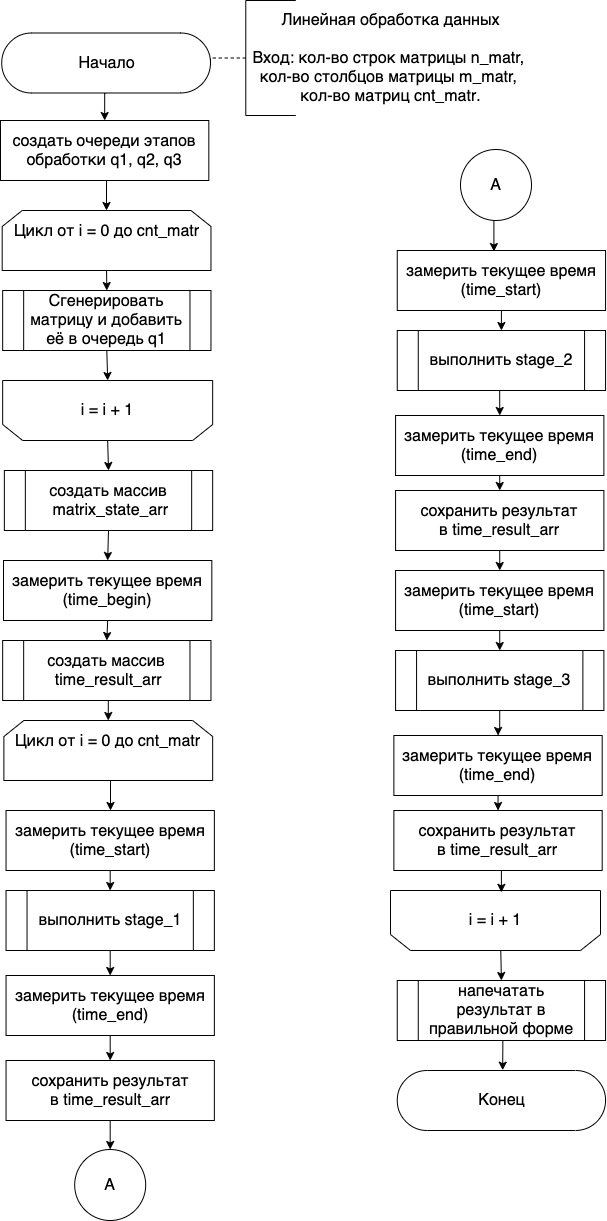
\includegraphics[scale=0.55]{img/linear_processing.png}
	\caption{Схема алгоритма линейной обработки матроицы}
	\label{fig:linear_processing}
\end{figure}

\clearpage

\begin{figure}[h]
	\centering
	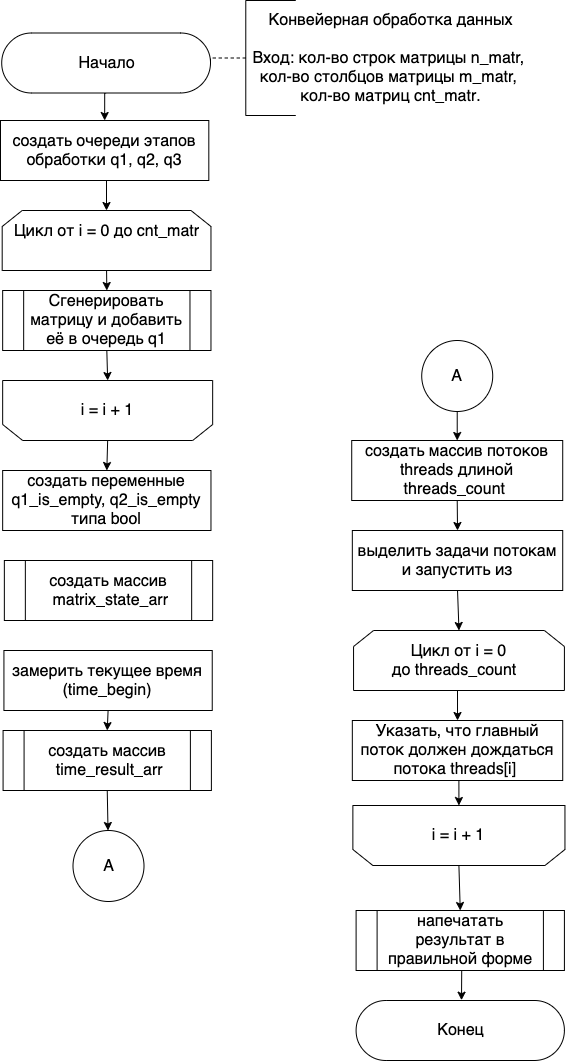
\includegraphics[scale=0.6]{img/parallel_processing.png}
	\caption{Схема алгоритма конвейерной обработки матроицы}
	\label{fig:parallel_processing}
\end{figure}

\clearpage

\begin{figure}[h]
	\centering
	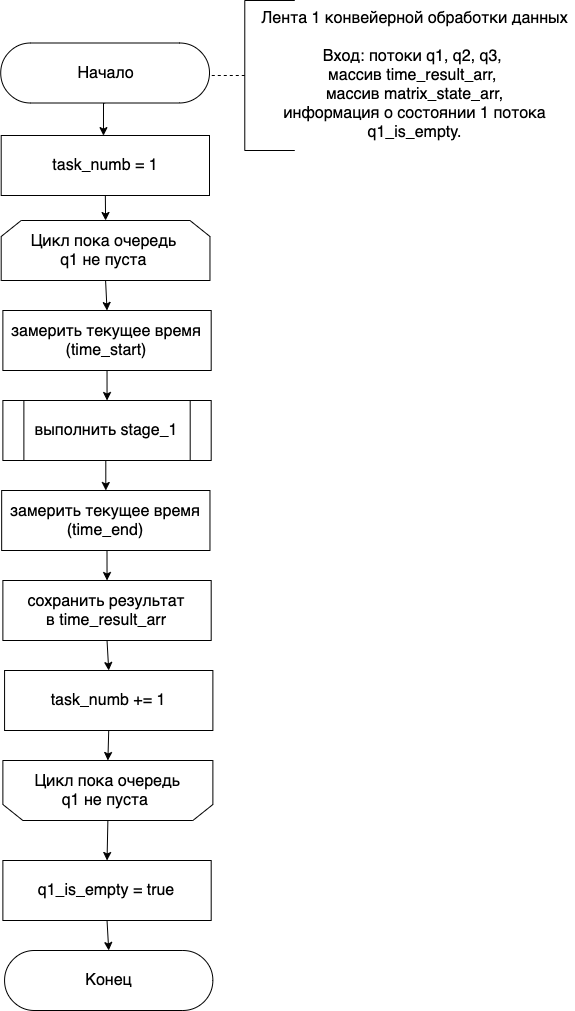
\includegraphics[scale=0.6]{img/parallel_stage_1.png}
	\caption{Схема 1-ой ленты конвейерной обработки матрицы}
	\label{fig:parallel_stage_1}
\end{figure} 

\clearpage

\begin{figure}[h]
	\centering
	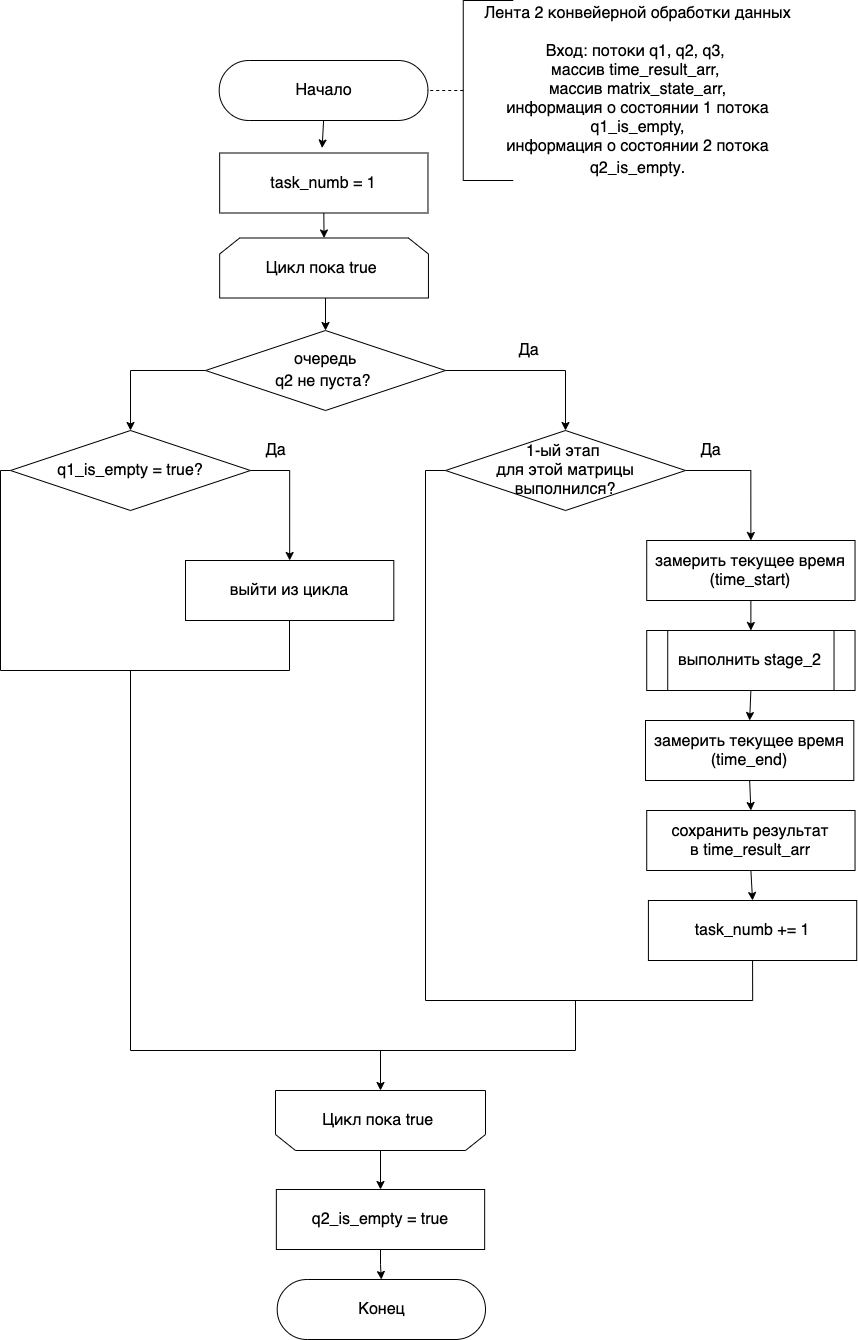
\includegraphics[scale=0.5]{img/parallel_stage_2.png}
	\caption{Схема 2-ой ленты конвейерной обработки матрицы}
	\label{fig:parallel_stage_2}
\end{figure} 

\clearpage

\begin{figure}[h]
	\centering
	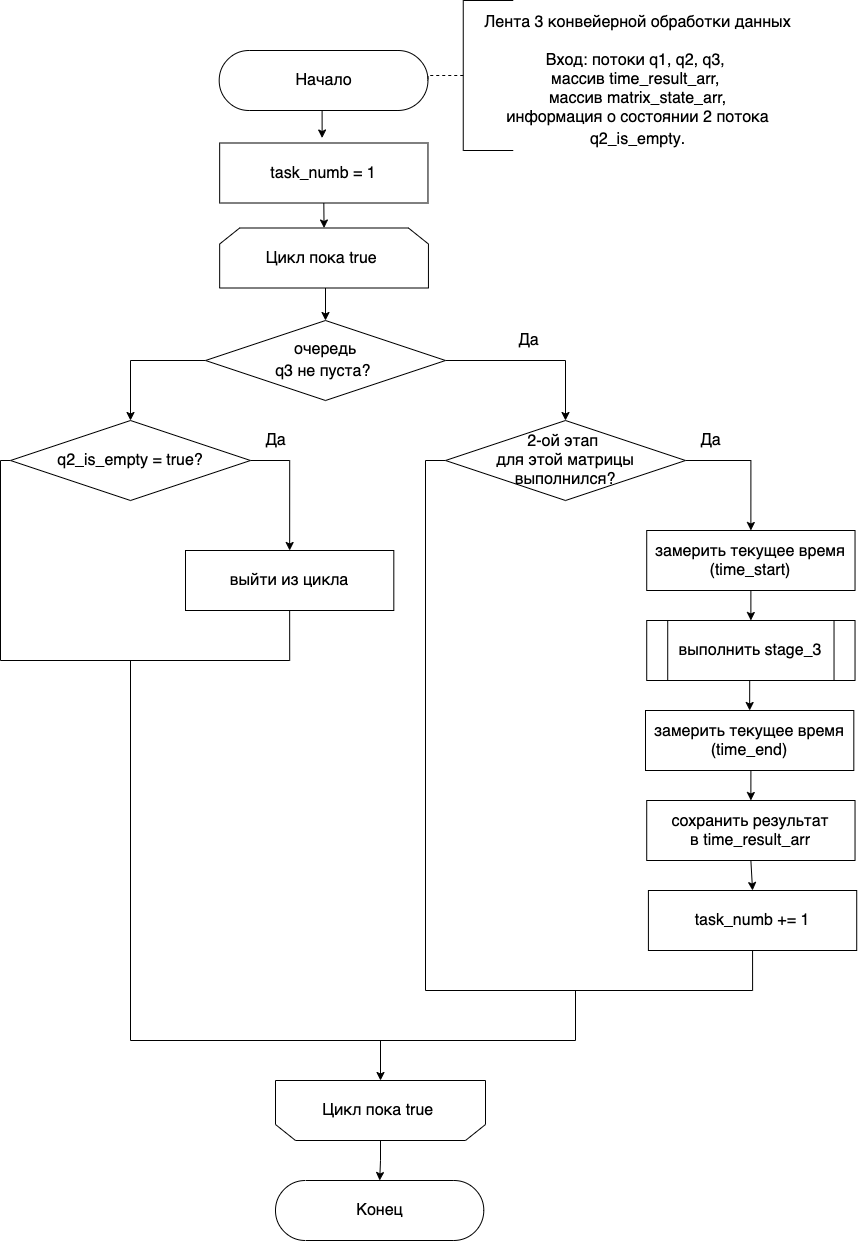
\includegraphics[scale=0.5]{img/parallel_stage_3.png}
	\caption{Схема 3-ей ленты конвейерной обработки матрицы}
	\label{fig:parallel_stage_3}
\end{figure} 

\clearpage

\begin{figure}[h]
	\centering
	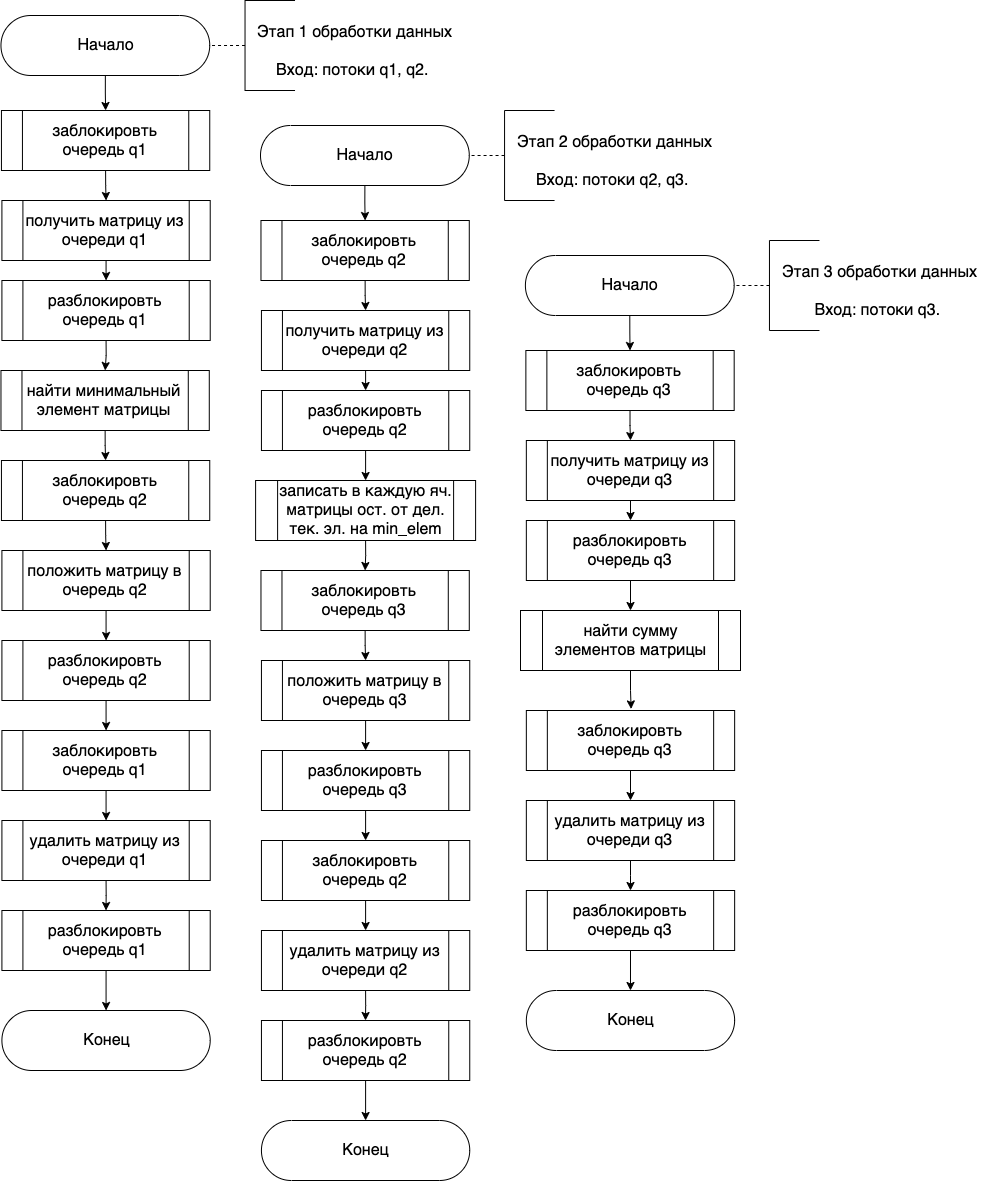
\includegraphics[scale=0.5]{img/stages.png}
	\caption{Схема реализаций этапов обработки матроицы}
	\label{fig:stages}
\end{figure} 

\clearpage

\section{Классы эквивалентности}

Выделенные классы эквивалентности для тестирования:

\begin{itemize}
	\item кол-во строк матрицы <= 0;
	\item кол-во столбцов матрицы <= 0;
	\item кол-во строк матрицы не является целым числом;
	\item кол-во столбцов матрицы не является целым числом;
	\item кол-во обрабатываемых матриц <= 0;
	\item кол-во обрабатываемых матриц не является целым числом;
	\item номер команды < 0 или > 3;
	\item номер команды не является целым числом;
	\item корректный ввод всех параметров;
\end{itemize}

\section{Описание используемых типов данных}

При реализации алгоритмов будут использованы следующие структуры данных:

\begin{itemize}
	\item кол-во матриц - целое число типа $int$;
	\item матрица - структура типа $matrix\_t$, имеющая следующие поля: 
	\begin{itemize}
		\item $std::vector<std::vector<int>>$ matr (сама матрица);
		\item $int$ n (кол-во строк в матрице);
		\item $int$ m (кол-во столбцов в матрице);
		\item $int$ min\_elem (минимальный элемент в изначальной матрице);
		\item $int$ sum\_elem (сумма элементов в конечной матрице);
	\end{itemize}
	\item очереди имеют тип $std::queue<matrix\_t>$;
	\item threads - массив потоков типа $std::thread$ размера 3;
	\item структура состояния матрицы $matrix\_state$, которая содержит информацию, какие из этапов обработки матрицы выполнились, имеет следующие поля: 
	\begin{itemize}
		\item $bool$ stage\_1 ($true$, если 1-ый этап выполнился);
		\item $bool$ stage\_2 ($true$, если 2-ой этап выполнился);
		\item $bool$ stage\_3 ($true$, если 3-ий этап выполнился);
	\end{itemize}
	\item время выполнения этапов обработки каждой матрицы записывается в массив типа $res\_time\_t$ ($struct$ result\_time), эта структура имеет следующие поля:
	\begin{itemize}
		\item $int$ task (номер матрицы на ленте);
		\item $int$ tape (номер ленты);
		\item $double$ beg (время начала обработки этой матрицы на этой ленте);
		\item $double$ end (время конца обработки этой матрицы на этой ленте);
		\item $std::chrono::time\_point<std::chrono::system\_clock>$ time\_begin (время начала обработки матриц);
	\end{itemize}
\end{itemize}

\clearpage

\section{Структура ПО}

ПО будет состоять из следующих модулей:

\begin{itemize}
	\item $main.cpp$ - файл, содержащий функцию $main$;
    \item $matrix.cpp$ - файл, содержащий функции для работы с матрицей;
    \item $compare.cpp$ - файл, в котором содержатся функции для замера времени работы алгоритмов;
    \item $read.cpp$ - файл, в котором содержатся функции ввода данных;
    \item $conveyor.cpp$ - файл, в котором содержатся функции для конвейерной и линейной обработок матриц;
    \item $errors.h$ - файл, в котором содержатся классы для всех ошибок, которые могут возникнуть во время работы программы;
    \item $color.h$ - файл, который содержит макросы для цветного вывода результата работы программы в консоль;
    \item $graph.py$ - файл, содержащий функции для построения графиков зависимости времени от размера и кол-ва матриц;
\end{itemize}

Каждый файл с расширением $.cpp$ имеет вспомогательный файл с расширением $.hpp$, где содержатся объявления функций, структуры, инклуды и дефайны.

\section{Вывод}

В данном разделе на основе теоретических данных были построены схемы требуемых методов обработки матриц (конвейерного и линейного), выбраны используемые типы данных, выделены классы эквивалентности для тестирования, а также была описана структура ПО.

\clearpage





\chapter{Технологическая часть}

В данном разделе будут приведены требования к программному обеспечению, средства реализации, листинги кода, а также функциональные тесты.

\section{Требования к программному обеспечению}

\begin{itemize}
    \item входные данные - кол-во строк и столбцов матрицы $matr$ должно быть > 0, все элементы матрицы имеют тип $int$, кол-во матриц > 0;
    \item выходные данные - табличка с номерами матриц, номерами этапов (лент) её обработки, временем начала обработки текущей матрицы на текущей ленте, временем окончания обработки текущей матрицы на текущей ленте.
\end{itemize}

\section{Средства реализации}

В данной работе для реализации был выбран язык программирования \textit{C++} [2]. Выбор обсуловлен наличием опыта работы с ним. Время работы было замерено с помощью функции \textit{std::chrono::system\_clock::now()} [3].

\clearpage

\section{Листинги кода}

В листингах \ref{lst:parallel_processing} - \ref{lst:stage_3} представлены функции для конвейерного и ленейного алгоритмов обработки матриц.

\begin{center}
\captionsetup{justification=raggedright,singlelinecheck=off}
\begin{lstlisting}[label=lst:parallel_processing,caption=Функция алгоритма конвейерной обработки матрицы]
void parallel_processing(int n_matr, int m_matr, int cnt_matr, bool matr_is_print, bool compare_time)
{
	std::queue<matrix_t> q1;
	std::queue<matrix_t> q2;
	std::queue<matrix_t> q3;

	std::mutex m;

	for (int i = 0; i < cnt_matr; i++)
	{
		matrix_t matr = generate_matrix(n_matr, m_matr);
		q1.push(matr);

		if (matr_is_print && i == cnt_matr - 1)
		{
			m.lock();
			printf("Первоначальная матрица:\n");
			print_matrix(matr);
			m.unlock();
		}
	}
	
	bool q1_is_empty = false;
	bool q2_is_empty = false;

	std::vector<matrix_state_t> matrix_state_arr;
	init_matrix_state_arr(matrix_state_arr, cnt_matr);

	std::chrono::time_point<std::chrono::system_clock> time_begin = 
	std::chrono::system_clock::now();

	std::vector<res_time_t> time_result_arr;
	init_time_result_arr(time_result_arr, time_begin, cnt_matr, THREADS_COUNT);

	std::thread threads[THREADS_COUNT];

	threads[0] = std::thread(parallel_stage_1, std::ref(q1), std::ref(q2), std::ref(time_result_arr), std::ref(matrix_state_arr), std::ref(q1_is_empty));
	threads[1] = std::thread(parallel_stage_2, std::ref(q2), std::ref(q3), std::ref(time_result_arr), std::ref(matrix_state_arr), std::ref(q1_is_empty), std::ref(q2_is_empty));
	threads[2] = std::thread(parallel_stage_3, std::ref(q3), std::ref(time_result_arr), std::ref(matrix_state_arr), std::ref(q2_is_empty), cnt_matr, matr_is_print);

	for (int i = 0; i < THREADS_COUNT; i++)
	{
		threads[i].join();
	}

	if (compare_time)
	{
		printf("     %4d      %s|%s     %4d      %s|%s   %.6f  \n",
			n_matr, PURPLE, BASE_COLOR, 
			cnt_matr, PURPLE, BASE_COLOR,
			time_result_arr[cnt_matr - 1].end);
	}
	else
	{
		print_res_time(time_result_arr, cnt_matr * THREADS_COUNT);
	}
}
\end{lstlisting}
\end{center}

\clearpage

\begin{center}
\captionsetup{justification=raggedright,singlelinecheck=off}
\begin{lstlisting}[label=lst:linear_processing,caption=Функция алгоритма линейной обработки матрицы]
void linear_processing(int n_matr, int m_matr, int cnt_matr, bool matr_is_print, bool compare_time)
{
	std::queue<matrix_t> q1;
	std::queue<matrix_t> q2;
	std::queue<matrix_t> q3;

	std::mutex m;

	for (int i = 0; i < cnt_matr; i++)
	{
		matrix_t matr = generate_matrix(n_matr, m_matr);
		q1.push(matr);

		if (matr_is_print && i == cnt_matr - 1)
		{
			m.lock();
			printf("Первоначальная матрица:\n");
			print_matrix(matr);
			m.unlock();
		}
	}

	std::vector<matrix_state_t> matrix_state_arr;
	init_matrix_state_arr(matrix_state_arr, cnt_matr);

	std::chrono::time_point<std::chrono::system_clock> time_start, time_end, 
	time_begin = std::chrono::system_clock::now();

	std::vector<res_time_t> time_result_arr;
	init_time_result_arr(time_result_arr, time_begin, cnt_matr, THREADS_COUNT);

	for (int i = 0; i < cnt_matr; i++)
	{
		time_start = std::chrono::system_clock::now();
		stage_1(std::ref(q1), std::ref(q2));
		time_end = std::chrono::system_clock::now();
		
		save_result(time_result_arr, time_start, time_end, time_begin, i + 1, 1);

		time_start = std::chrono::system_clock::now();
		stage_2(std::ref(q2), std::ref(q3));
		time_end = std::chrono::system_clock::now();

		save_result(time_result_arr, time_start, time_end, time_begin, i + 1, 2);

		time_start = std::chrono::system_clock::now();
		stage_3(std::ref(q3), i + 1, cnt_matr, matr_is_print);
		time_end = std::chrono::system_clock::now();

		save_result(time_result_arr, time_start, time_end, time_begin, i + 1, 3);
	}

	if (compare_time)
	{
		printf("     %4d      %s|%s     %4d      %s|%s   %.6f  \n",
			n_matr, PURPLE, BASE_COLOR, 
			cnt_matr, PURPLE, BASE_COLOR,
			time_result_arr[cnt_matr - 1].end);
	}
	else
	{
		print_res_time(time_result_arr, cnt_matr * THREADS_COUNT);
	}
}
\end{lstlisting}
\end{center}


\begin{center}
\captionsetup{justification=raggedright,singlelinecheck=off}
\begin{lstlisting}[label=lst:parallel_stage_1,caption=Функция 1-ой ленты конвейерной обработки матрицы]
void parallel_stage_1(std::queue<matrix_t> &q1, std::queue<matrix_t> &q2,
                      std::vector<res_time_t> &time_result_arr,
                      std::vector<matrix_state_t> &matrix_state_arr, 
                      bool &q1_is_empty)
{
    std::chrono::time_point<std::chrono::system_clock> time_start, time_end;
    int task_num = 1;

    while(!q1.empty())
    {   
        time_start = std::chrono::system_clock::now();
        stage_1(std::ref(q1), std::ref(q2));
        time_end = std::chrono::system_clock::now();

        save_result(time_result_arr, time_start, time_end, time_result_arr[0].time_begin, task_num, 1);

        matrix_state_arr[task_num - 1].stage_1 = true;
        task_num++;
    }

    q1_is_empty = true;
}
\end{lstlisting}
\end{center}

\clearpage

\begin{center}
\captionsetup{justification=raggedright,singlelinecheck=off}
\begin{lstlisting}[label=lst:parallel_stage_2,caption=Функция 2-ой ленты конвейерной обработки матрицы]
void parallel_stage_2(std::queue<matrix_t> &q2, std::queue<matrix_t> &q3,
                      std::vector<res_time_t> &time_result_arr,
                      std::vector<matrix_state_t> &matrix_state_arr, 
                      bool &q1_is_empty, bool &q2_is_empty)
{
    std::chrono::time_point<std::chrono::system_clock> time_start, time_end;
    int task_num = 1;

    while(true)
    {      
        if (!q2.empty())
        {   
            if (matrix_state_arr[task_num - 1].stage_1 == true)
            {
                time_start = std::chrono::system_clock::now();
                stage_2(std::ref(q2), std::ref(q3));
                time_end = std::chrono::system_clock::now();

                save_result(time_result_arr, time_start, time_end, time_result_arr[0].time_begin, task_num, 2);

                matrix_state_arr[task_num - 1].stage_2 = true;
                task_num++;
            }
        }
        else if(q1_is_empty)
        {
            break;
        }
    }

    q2_is_empty = true;
}
\end{lstlisting}
\end{center}

\clearpage

\begin{center}
\captionsetup{justification=raggedright,singlelinecheck=off}
\begin{lstlisting}[label=lst:parallel_stage_3,caption=Функция 3-ей ленты конвейерной обработки матрицы]
void parallel_stage_3(std::queue<matrix_t> &q3, 
                      std::vector<res_time_t> &time_result_arr,
                      std::vector<matrix_state_t> &matrix_state_arr, 
                      bool &q2_is_empty, int cnt_matr, bool matr_is_print)
{
    std::chrono::time_point<std::chrono::system_clock> time_start, time_end;
    int task_num = 1;

    while(true)
    {      
        if (!q3.empty())
        {   
            if (matrix_state_arr[task_num - 1].stage_2 == true)
            {
                time_start = std::chrono::system_clock::now();
                stage_3(std::ref(q3), task_num, cnt_matr, matr_is_print);
                time_end = std::chrono::system_clock::now();

                save_result(time_result_arr, time_start, time_end, time_result_arr[0].time_begin, task_num, 3);

                matrix_state_arr[task_num - 1].stage_3 = true;
                task_num++;
            }
        }
        else if(q2_is_empty)
        {
            break;
        } 
    }
}
\end{lstlisting}
\end{center}

\clearpage

\begin{center}
\captionsetup{justification=raggedright,singlelinecheck=off}
\begin{lstlisting}[label=lst:stage_1,caption=Функция реализации 1-ого этапа обработки матрицы]
void stage_1(std::queue<matrix_t> &q1, std::queue<matrix_t> &q2)
{
	std::mutex m;

	m.lock();
	matrix_t matr = q1.front();
	m.unlock();

	matr.min_elem = get_min_elem(matr);

	m.lock();
	q2.push(matr);
	m.unlock();

	m.lock();
	q1.pop();
	m.unlock();
}
\end{lstlisting}
\end{center}

\begin{center}
\captionsetup{justification=raggedright,singlelinecheck=off}
\begin{lstlisting}[label=lst:stage_2,caption=Функция реализации 2-ого этапа обработки матрицы]
void stage_2(std::queue<matrix_t> &q2, std::queue<matrix_t> &q3)
{
	std::mutex m;

	m.lock();
	matrix_t matr = q2.front();
	m.unlock();

	mod_by_min_elem(matr);
	
	m.lock();
	q3.push(matr);
	m.unlock();
	
	m.lock();
	q2.pop();
	m.unlock();
}
\end{lstlisting}
\end{center}

\clearpage

\begin{center}
\captionsetup{justification=raggedright,singlelinecheck=off}
\begin{lstlisting}[label=lst:stage_3,caption=Функция реализации 3-его этапа обработки матрицы]
void stage_3(std::queue<matrix_t> &q3, int task_num, int cnt_matr, bool matr_is_print)
{
	std::mutex m;

	m.lock();
	matrix_t matr = q3.front();
	m.unlock();

	matr.sum_elem = get_sum_elements(matr);
	
	if (matr_is_print && task_num == cnt_matr)
	{
		printf("\nmin_elem = %d\n\nМатрица после 2 этапа:\n", matr.min_elem);        
		print_matrix(matr);
		printf("\nsum_elem = %d\n\n", matr.sum_elem);
	}

	m.lock();
	q3.pop();
	m.unlock();
}
\end{lstlisting}
\end{center}

\clearpage

\section{Функциональные тесты}

В таблице \ref{tbl:functional_test} приведены функциональные тесты для конвейерного и ленейного алгоритмов обработки матриц. Все тесты пройдены успешно.

\begin{table}[h]
	\begin{center}
	\begin{threeparttable}
		\captionsetup{justification=raggedright,singlelinecheck=off}
		\caption{\label{tbl:functional_test} Функциональные тесты}
		\begin{tabular}{|c|c|c|c|c|}
			\hline
			Строк & Столбцов & Метод обр. & Алгоритм & Ожидаемый результат 
			\\ \hline
			0 & 10 & 10 & Конвейерный & Сообщение об ошибке 
			\\ \hline
			k & 10 & 10 & Конвейерный & Сообщение об ошибке 
			\\ \hline
			10 & 0 & 10 & Конвейерный & Сообщение об ошибке 
			\\ \hline
			10 & k & 10 & Конвейерный & Сообщение об ошибке 
			\\ \hline
			10 & 10 & -5 & Конвейерный & Сообщение об ошибке 
			\\ \hline
			10 & 10 & k & Конвейерный & Сообщение об ошибке 
			\\ \hline
			100 & 100 & 20 & Конвейерный & Вывод результ. таблички
			\\ \hline
			100 & 100 & 20 & Линейный & Вывод результ. таблички
			\\ \hline
			50 & 100 & 100 & Линейный & Вывод результ. таблички
			\\ \hline
		\end{tabular}
	\end{threeparttable}
	\end{center}
\end{table}

\section{Вывод}

В данном разделе были разработаны алгоритмы для конвейерного и ленейного алгоритмов обработки матриц, проведено тестирование, описаны средства реализации и требования к ПО.





\chapter{Исследовательская часть}

\section{Технические характеристики}

Технические характеристики устройства, на котором выполнялось тестирование представлены далее.

\begin{itemize}
    \item Операционная система: macOS 11.5.2. [4]
    \item Память: 8 GiB.
    \item Процессор: 2,3 GHz 4‑ядерный процессор Intel Core i5. [5]
\end{itemize}

При тестировании ноутбук был включен в сеть электропитания. Во время тестирования ноутбук был нагружен только встроенными приложениями окружения, а также системой тестирования.

\clearpage

\section{Демонстрация работы программы}

\img{220mm}{example_parallel}{Пример работы программы (конвейерная реализация)}

\clearpage

\img{220mm}{example_linear}{Пример работы программы (линейная реализация)}

\clearpage

\section{Время выполнения алгоритмов}

Результаты замеров времени работы алгоритмов обработки матриц для конвейерной и ленейной реализаций представлены на рисунках 4.3 - 4.5. Замеры времени проводились в секундах и усреднялись для каждого набора одинаковых экспериментов.

\img{180mm}{time}{Замеры времени работы алгоритмов для конвейерной и ленейной реализаций}

\img{110mm}{graph_diff_quantities}{Зависимость времени работы алгоритмов от кол-ва матриц (размеры матриц 100х100)}

\img{110mm}{graph_diff_sizes}{Зависимость времени работы алгоритмов от размера матриц (кол-во матриц = 100)}

\clearpage

\section{Вывод}

В этом разделе были указаны технические характеристики машины, на которой происходило сравнение времени работы алгоритмов обработки матриц для конвейерной и ленейной реализаций.

В результате замеров времени было установлено, что конвейерная реализация обработки лучше линейной
при большом кол-ве матриц (в 2.5 раза при 400 матрицах, в 2.6 раза при 800 и в 2.7 при 1600). Так же конвейерная обработка показала себя лучше при увеличении размеров обрабатываемых матриц (в 2.8 раза при размере матриц 160х160, в 2.9 раза при размере 320х320 и в 2.9 раза при матрицах 640х640). Значит при большом кол-ве обрабатываемых матриц, а так же при матрицах большого размера стоит использовать конвейерную реализацию обработки, а не линейную.





\chapter*{Заключение}
\addcontentsline{toc}{chapter}{Заключение}

Было экспериментально подтверждено различие во временной эффективности конвейрной и линейной реализаций обработак матриц. В результате исследований можно сделать вывод о том, что при большом кол-ве обрабатываемых матриц, а так же при матрицах большого размера стоит использовать конвейерную реализацию обработки, а не линейную (при 1600 матриц конвейерная быстрее в 2.7 раза, а при матрицах 640х640 быстрее в 2.9 раза).

\vspace{5mm}

В ходе выполнения данной лабораторной работы были решены следующие задачи:
\begin{itemize}
	\item изучены основы конвейерной обработки данных;
	\item применены изученные основы для реализации конвейерной обработки матриц;
	\item произведен сравнительный анализ линейной и конвейерной реализаций обработки матриц;
	\item экспериментально подтверждено различие во временнoй эффективности линейной и конвейерной реализаций обработки матриц при помощи разработанного программного обеспечения на материале замеров процессорного времени;
	\item описаны и обоснованы полученные результаты в отчете о выполненной лабораторной работе.
\end{itemize}

Поставленная цель была достигнута.





\begin{thebibliography}{5}
	\bibitem{bib1}
	Конвейерная организация [Электронный ресурс]. Режим доступа: \url{http://www.citforum.mstu.edu.ru/hardware/svk/glava_5.shtml} (дата обращения: 01.12.2021).
	\bibitem{bib2}
	C++ –– Типизированный язык программирования / Хабр [Электронный ресурс]. Режим доступа: \url{https://habr.com/ru/hub/cpp/} (дата обращения: 20.10.2021).
	\bibitem{bib3}
	std::chrono::system\_clock::now - cppreference.com [Электронный ресурс]. Режим доступа: \url{https://en.cppreference.com/w/cpp/chrono/system_clock/now} (дата обращения: 20.10.2021).
	\bibitem{bib4}
	macOS Monterey - Apple(RU) [Электронный ресурс]. Режим доступа: \url{https://www.apple.com/ru/macos/monterey/} (дата обращения: 14.10.2021).
	\bibitem{bib5}
	Intel [Электронный ресурс]. Режим доступа: \url{https://www.intel.ru/content/www/ru/ru/products/details/processors/core/i5.html} (дата обращения: 14.10.2021).
\end{thebibliography}

\addcontentsline{toc}{chapter}{Список литература}

\end{document}
